\documentclass[conference]{IEEEtran}

\IEEEoverridecommandlockouts

\input{glyphtounicode}
\pdfgentounicode=1
\usepackage{cmap}
\usepackage[T1]{fontenc}
\usepackage{textcomp}
\usepackage{amsmath,amssymb,bm}
\usepackage{graphicx}
\usepackage{booktabs}
\usepackage{array}
\usepackage{multirow}
\usepackage{cite}
\usepackage{url}
\usepackage{xcolor}

\graphicspath{{figures/}}
\raggedbottom
\setlength{\textfloatsep}{6pt plus 1pt minus 1pt}
\setlength{\floatsep}{5pt plus 1pt minus 1pt}
\setlength{\dbltextfloatsep}{6pt plus 1pt minus 1pt}
\setlength{\dblfloatsep}{5pt plus 1pt minus 1pt}
\setlength{\abovedisplayskip}{4pt plus 1pt minus 1pt}
\setlength{\belowdisplayskip}{4pt plus 1pt minus 1pt}
\setlength{\abovecaptionskip}{3pt plus 1pt minus 1pt}
\setlength{\belowcaptionskip}{0pt plus 1pt minus 1pt}

\newcommand{\MPC}{\mathrm{MPC}}
\newcommand{\VLM}{\mathrm{VLM}}
\newcommand{\distw}{d_{\mathrm{world}}}
\newcommand{\pass}{\textsc{pass}}
\newcommand{\fail}{\textsc{fail}}

\title{Traceable Reproduction Audit and Feedback-Assisted Diagnostics\\
for VLMPC-Style Language-Table Pushing}


\author{%
\IEEEauthorblockN{Xiao Yi}
\IEEEauthorblockA{\textit{College of Computer Science and Technology}\\
\textit{Tongji University}\\
Shanghai, China}
\and
\IEEEauthorblockN{Yuanqiang Zhou}
\IEEEauthorblockA{\textit{Department of Control Science and Engineering}\\
\textit{College of Electronics and Information Engineering}\\
\textit{Tongji University}\\
Shanghai, China}
}

\begin{document}
\maketitle

\begin{abstract}
  Vision-language model predictive control (VLMPC) links semantic perception with receding-horizon control, but a reproduction study must distinguish an executable implementation from reliable closed-loop behavior. This paper audits a VLMPC-style Language-Table pushing system under a traceable protocol covering multi-seed controller reruns, language and image inputs, parameter ablations, event-triggered VLM re-query, target-image grounding, and visual-feedback boundaries. A fresh four-variant raw-MPC sweep over seeds 45--48 contains 16 runs and obtains 0/16 successes at the $\distw^{\mathrm{final}}\leq0.08$ evaluation tolerance; the archived eight-run parameter ablation also remains at 0/8. Feedback-assisted diagnostics use privileged simulator-state feedback: grounded original MPC obtains 4/4 and 8/8 diagnostic successes, with 23/23 raw planner actions replaced in all 12 runs, while the latest semantic-MPC suite obtains 18/18 selected-target control successes with mean final distance $0.0641\pm0.0150$ (sample SD). Its 18 rows are partitioned into 15/15 fixed-target controls, one natural-language instruction with 1/1 instruction-level joint success, one target-image selected-target control, and one free scene-selection control. Only the natural-language row is instruction-evaluable; the single target-image row is not an independent image-grounding test. A fresh target-image matrix covers three cases and seeds 42--44: semantic selection and joint active control each succeed in 8/9 trials, including one retained yellow-pentagon selection failure. A new independent CodexCLIClient audit covers three instructions and seeds 42--44, with 9/9 independently checked target selections and 9/9 joint controls under strict no-cache mode. Fresh matched event controls show that natural re-query executes in 3/3 enabled trials but leaves final distances identical to no-event controls; an expanded six-seed forced semantic-fault audit repairs the target in 6/6 trials and reaches the true-target threshold in 5/6, versus 0/6 for controls. A detector/tracker visual-feedback implementation is also tested and fails in 0/6 trials, with mean final distance $0.3160\pm0.1439$. The resulting contribution is a negative raw-reproduction audit plus bounded diagnostic evidence, not a benchmark-level proof of unmodified VLMPC success.
\end{abstract}

\begin{IEEEkeywords}
Vision-language model predictive control, semantic MPC, Language-Table, reproduction audit, event re-query, target-image grounding.
\end{IEEEkeywords}

\section{Introduction}
Robotic manipulation systems increasingly need to connect semantic understanding, visual perception, and closed-loop control. A table-top pushing task appears simple, yet a successful controller must recognize the relevant object, ground the goal, choose a feasible push direction, recover from perception drift, and stop near the target region. Model predictive control (MPC) is useful in such settings because it repeatedly predicts future states, optimizes candidate controls, and executes only the first action before replanning \cite{mayne2000mpc,rawlings2017mpc}. Classical MPC, however, usually assumes that state variables and objectives are already available. Vision-language models (VLMs) and vision-language-action systems add semantic grounding and instruction understanding \cite{ahn2022saycan,brohan2023rt2,huang2022inner}, but they still require reliable low-level control to produce stable physical behavior.

VLMPC aims to bridge these two sides by placing VLM-based semantic evaluation inside a visual MPC loop \cite{zhao2024vlmpc}. The original framework takes a goal image or language instruction, samples candidate action sequences, predicts future visual observations, and evaluates the predictions with a hierarchical cost. Later trajectory-level variants further suggest that reducing the burden of video prediction can improve long-horizon manipulation planning \cite{chen2025trajvlmpc}. For a constrained local reproduction study, the key question is therefore not only whether the program can run, but what experimental evidence supports each success claim.

 This paper summarizes our study around that question. We use Language-Table push-to-corner tasks and evaluate the unmodified video-prediction MPC chain, grounded and semantic oracle-feedback diagnostics, a target-image interface, event-triggered VLM re-query, and a detector/tracker visual-feedback boundary test. The central reporting choice is to keep negative results visible. The fresh unmodified sweep is executable and logged, but remains unsuccessful across all 16 controller-variant/seed combinations. The positive 4/4, 8/8, and selected-target 18/18 numbers come from feedback-assisted diagnostic paths and are therefore reported with an explicit state-source and target-reference flag; the semantic suite is partitioned into 15 fixed-target controls, one natural-language instruction (the only instruction-evaluable row), one target-image interface control, and one free scene-selection control. In contrast, the visual-feedback implementation is tested without simulator-state access and also fails in 0/6 trials. This separation prevents an oracle-stabilized engineering path from being mistaken for a faithful reproduction of the original video-prediction controller or for a solved visual-feedback system.

The contributions are:
\begin{enumerate}
\setlength{\itemsep}{0pt}
\item A traceable reproduction audit of a VLMPC-style Language-Table manipulation chain, including unmodified controller comparison and original parameter ablation.
\item A conservative symptom analysis that connects failed runs to logged tracking jumps, visual-prediction/control mismatch, parameter sensitivity, and absence of final-action feedback, without claiming single-factor causality.
\item Two bounded diagnostic enhancements: grounded original MPC, which preserves raw planner calls but applies final action correction, and semantic MPC, which combines semantic target selection with state-feedback pushing.
\item A branch-level accounting of planner authority, including the grounded branch's raw-action replacement rate and the semantic branch's zero active raw-sampling budget.
 \item A file-traceable experimental package with sanitized per-run and aggregate CSVs, publication figures, qualitative frames, matched event controls, a repeated target-image end-to-end matrix, a visual-feedback boundary test, and a controlled semantic-fault re-query audit.
\end{enumerate}

\section{Related Work}
\subsection{Visual MPC and Video-Prediction Control}
Visual MPC uses learned visual dynamics to support model-based manipulation directly in image space. Deep visual foresight and related visual MPC systems showed that action-conditioned video prediction can guide robot motion without a hand-designed dynamics model \cite{finn2017deep,ebert2018visual}. Such approaches are attractive for open-ended manipulation, but they are also sensitive to prediction bias, object occlusion, and long-horizon compounding errors. These limitations are relevant to our reproduction: the planner can generate candidate futures and rank actions, but the unmodified closed loop does not reliably drive the object to the selected goal region.

\subsection{Vision-Language Manipulation}
Language-conditioned manipulation has used VLMs and language models for task grounding, affordance selection, reasoning, and failure interpretation. CLIPort separates semantic ``what'' reasoning from spatial ``where'' execution \cite{shridhar2021cliport}. SayCan grounds language plans with affordances \cite{ahn2022saycan}. Inner Monologue emphasizes feedback-aware embodied reasoning \cite{huang2022inner}, and VoxPoser composes 3D value maps for robotic manipulation from language-model reasoning \cite{huang2023voxposer}. These systems motivate our use of explicit feedback and event handling: semantic decisions must be connected to low-level execution evidence, not only to high-level task labels.

\subsection{VLMPC, Trajectory Variants, and Testing}
VLMPC integrates VLM perception with MPC-style candidate action evaluation \cite{zhao2024vlmpc}. Traj-VLMPC further reduces computational overhead by using trajectory generation rather than full video prediction \cite{chen2025trajvlmpc}. At the same time, evaluation work such as VLATest argues that VLM/VLA manipulation systems require robustness and reliability tests beyond isolated demonstrations \cite{wang2024vlatest}. Failure-reasoning systems such as AHA also show the value of identifying manipulation failure modes \cite{duan2024aha}. Our work follows this evaluation-oriented line: we do not hide failed unmodified runs, and we mark diagnostic controllers that use privileged state feedback.

\section{Evaluation Setup and Evidence Sources}
\subsection{Task Definition}
The experiment uses Language-Table desktop pushing tasks. A target object such as \emph{red moon}, \emph{blue cube}, or \emph{yellow pentagon} should be pushed toward a designated corner. The controller input can be a fixed target label, a natural-language instruction, a target image, or a VLM-based scene selection request. The action is a planar end-effector push in the simulated table environment.

The primary metric is the final world-coordinate distance between the target object and the goal:
\begin{equation}
  \mathrm{success} = \mathbb{I}\left[\distw^{\mathrm{final}} \leq 0.08\right].
  \label{eq:success}
\end{equation}
The threshold 0.08 is an evaluation tolerance used consistently in the archived final runs, not a universal manipulation success criterion. Threshold sensitivity changes the interpretation of the positive results: at 0.05, the archived grounded diagnostic suites drop to 0/4 and 0/8, and the latest semantic MPC suite succeeds in only 3/18 runs. We therefore report success rates primarily as evidence of coarse task completion under the evaluation tolerance, not precision placement.

For the live semantic suite, the distance-based control label is computed relative to the selected target recorded for that diagnostic condition. The 18 heterogeneous rows are partitioned by evaluation scope: 15 fixed-target controls, one natural-language instruction, one target-image interface row, and one free scene-selection row. Only the natural-language row is instruction-evaluable and it preserves the requested-to-selected identity and satisfies the instruction-level joint criterion (1/1). The fixed-target, target-image, and scene-selection rows are retained as separate selected-target controls (15/15, 1/1, and 1/1); the single target-image row is not an independent image-grounding test. The reported 18/18 value is therefore a conditional selected-target control result, not an end-to-end instruction or target-image grounding rate.

For the new target-image matrix, we distinguish a \emph{pre-satisfied} run, for which the true target is already within the threshold before the first action, from an \emph{active control} trial, which starts outside the threshold and executes at least one action. \emph{Joint active success} requires both correct target-image semantic selection and active control success. This prevents a zero-step terminal state from being counted as controller evidence.

\subsection{Evidence Artifacts}
All numerical results in this paper are extracted from the study package. The main evidence files are:
\begin{itemize}
\setlength{\itemsep}{0pt}
\item sanitized per-run and aggregate CSVs for the fresh raw-MPC sweep, semantic suite, target-image matrix, event controls, semantic-fault audit, and visual-feedback test;
\item supplement CSVs for exact method parameters, checkpoint/code hashes, target-image selection, and VLM cache status;
\item publication figures and selected qualitative frames used as visual evidence; raw service logs and videos remain outside the sanitized public package;
\item a portable robustness-edge audit CSV covering occlusion, viewpoint proxy, brightness shift, and unknown-target rejection, together with its four input images.
\end{itemize}
  The reporting goal is to make every claim traceable to these artifacts rather than to a post-hoc manual description. The formal revision runs use the project's \texttt{CodexCLIClient} with the \texttt{codex} backend and model alias GPT-5.5; credentials are supplied through an isolated \texttt{CODEX\_HOME} profile and are excluded from the manuscript and sanitized package. The revision controls use strict no-cache mode and record zero cache hits. They still do not prove that natural re-query causes recovery because matched no-event controls also succeed. The public repository is available at \url{https://github.com/yixiaogithub66/vlmpc-language-table-reproduction-audit}; the accompanying v1.0.8 artifact contains the authoritative result files, including the robustness-edge CSV and portable inputs, reproduction guide, parameter records, publication-figure source and exports, separate runtime-asset and source-snapshot manifests, and a reviewer-facing source snapshot. Third-party model weights are not redistributed and must be obtained from their original sources.

\section{Method}
\subsection{Unmodified Reproduction Chain}
The unmodified reproduction follows a VLMPC-style loop. A task input is grounded to a target, candidate action sequences are sampled, a visual prediction model forecasts future observations, and a cost function ranks the candidates before the first action is executed. Controller comparison includes baseline, improved, literature, and literature-v2 settings. Parameter ablation varies sampling budget and cost settings.

In this branch, no final-action state-feedback correction is applied. This distinction is crucial: these runs represent the closest archived reproduction of the original video-prediction MPC chain in our project, and they are evaluated separately from later enhancements.

\subsection{Codex CLI VLM Adapter}
The formal online VLM calls use the local \texttt{CodexCLIClient}, rather than a direct application-side HTTP request. For each \texttt{complete(prompt, image\_paths)} call, the adapter stages image attachments in an ASCII-only temporary directory when the project path contains non-ASCII characters, sends the prompt through standard input, and launches an ephemeral CLI request equivalent to
\begin{center}
\texttt{codex exec --skip-git-repo-check --ephemeral --color never}\newline
\texttt{-C <ASCII workdir> -o <temporary output> -m gpt-5.5 -i <image>}
\end{center}
The response is read from the temporary output file and then parsed for target, subtask, or re-query state. The adapter passes the isolated \texttt{CODEX\_HOME} environment to the child process and requires its \texttt{config.toml}; it does not place credentials in Python source. A cache, when explicitly enabled, is keyed by the model/configuration, prompt, and image-content hashes. The reported event controls disable this cache and record zero cache hits. The project also contains a direct OpenAI-compatible backend for development, but it was not used for the formal results; the CSV label ``responses-compatible'' describes the adapter response schema, not a claim that the final runs called the HTTP \texttt{/responses} endpoint.

\subsection{Archived Implementation Parameters}
Table~\ref{tab:methodparams} summarizes the recoverable implementation parameters. The unmodified planner uses horizon $H=20$, action dimension 2, and a correlated-noise sampler with $\beta=0.5$. The command-line defaults are 200 samples and replan frequency 5, while the archived ablation set contains eight logged configurations rather than a complete $3\times3$ grid. The literature-style cost is
\begin{equation}
\begin{split}
J ={}& d_{\mathrm{obj,goal}} + 0.35d_{\mathrm{contact}} +0.15d_{\mathrm{arm,obj}}
 + 18.0J_{\mathrm{align}}  \\
&+24.0J_{\mathrm{obs}} -1.2\Delta d
 + 12.0\mathbb{I}[\Delta d < 1.0],
\end{split}
\label{eq:cost}
\end{equation}
with obstacle decay 42 pixels. In the close-range branch, the contact, alignment, progress-reward, and non-progress terms are changed to 0.10, 6.0, 1.8, and 20.0, respectively. These values are implementation parameters recovered from \texttt{vlmpc.py}, not tuned benchmark claims.

\begin{table}[!t]
\centering
\caption{Recoverable implementation parameters from code, metrics, and supplement CSVs.}
\label{tab:methodparams}
\scriptsize
\begin{tabular}{@{}p{0.33\columnwidth}@{\hspace{4pt}}p{0.63\columnwidth}@{}}
\toprule
Parameter & Value or rule used in the combined audit \\
\midrule
Environment & BLOCK\_8 Language-Table, 10 Hz; fresh raw sweep uses seeds 45--48; semantic, target-image, and event controls use 42--44; visual feedback uses 45--50 \\
Raw MPC & action dim. 2, horizon 20; sampled candidates clipped to $[-0.02,0.02]$, executed action/feedback bound $[-0.08,0.08]$ \\
Budgets & default 200/5 samples/plan frequency; eight archived ablations: pf1/ns5, pf2/ns5, pf2/ns10, pf3/ns10, pf2/ns15, cost history low, cost default, cost target high \\
Detector/tracker & YOLO conf. 0.5; PySOT SiamRPN tracker \\
Cost weights & contact/approach/alignment/obstacle $=0.35/0.15/18.0/24.0$ \\
Progress terms & reward 1.2, non-progress penalty 12.0, min gain 1.0, obstacle decay 42 px \\
Close range & distance 135 px; contact/alignment/reward/penalty $=0.10/6.0/1.8/20.0$ \\
Feedback push & contact offset 0.06, clearance 0.12, move step 0.06, push step 0.075, tolerance 0.018 \\
Original event & default window/min-progress/min-step $=3/1.0/3$; semantic matched controls use $4/0.002/3$ with min progress in world-distance units \\
Semantic event & window 4, min progress 0.002 world-distance units, distance floor $1.5\times$ success distance \\
Online VLM & CodexCLIClient; local \texttt{codex exec -m gpt-5.5}; isolated \texttt{CODEX\_HOME}; credentials excluded \\
Success threshold & evaluation tolerance $\distw\leq0.08$; strict audit also reports 0.05 and 0.10 \\
\bottomrule
\end{tabular}
\end{table}

The runtime-asset manifest records SHA-256 prefixes for the externally obtained video-prediction, detector, and tracker assets. The source manifest separately records the executed-source and public-snapshot hashes. Five listed Python files are byte-identical. For \texttt{main.py}, the executed-source prefix is \texttt{d8078e7cba86} and the public-snapshot prefix is \texttt{f98caece7442}; the difference is limited to replacing a drive-local dependency fallback with environment-based configuration, without changing controller logic.

\subsection{Grounded Original MPC}
Grounded original MPC is a diagnostic enhancement. The raw planner path still runs, and raw MPC actions are recorded. After the raw action is obtained, a simulator-state feedback push correction is used for the executed action. The correction is bounded by action clipping and uses object, end-effector, and goal positions available from the simulator state. Across the 12 grounded runs (4 controller-comparison runs and 8 ablation runs), the logs contain 23 raw planner actions and 23 feedback overrides per run: the executed-action replacement rate is therefore 23/23, or 100\%, in every run. The raw planner remains useful for traceability and branch comparison, but it is not the authority over the executed action in this diagnostic branch.

The grounded and semantic branches use simulator-state feedback and therefore answer a diagnostic question rather than a reproduction question. The feedback action uses object, end-effector, and goal positions from simulator state. Let $\hat{d}_{\mathrm{push}}=(x_{\mathrm{goal}}-x_{\mathrm{obj}})/\|x_{\mathrm{goal}}-x_{\mathrm{obj}}\|$ and $x_{\mathrm{contact}}=x_{\mathrm{obj}}-0.06\hat{d}_{\mathrm{push}}$. The controller first stages the end effector near a side-clearance point, then moves to contact, and finally pushes:
\begin{equation}
  u_t = \mathrm{clip}\left(\alpha \hat{d}_{\mathrm{push}} +
  \beta(x_{\mathrm{contact}} - x_{\mathrm{ee}}), -0.08, 0.08\right).
  \label{eq:feedback}
\end{equation}
In the push phase, $\alpha=0.075$ and $\beta=0.45$; the stage/contact phases instead use a step-limited move of at most 0.06.

\subsection{Semantic MPC}
Semantic MPC is a second diagnostic path. It uses semantic target selection from fixed labels, language instructions, target images, or VLM scene selection, and then performs low-level pushing with state feedback. The strict repair adds an \texttt{auto|vlm|vision} target-image selector: in \texttt{auto} mode the system sends the target image and the current scene image to the configured VLM and asks it to choose among visible scene candidates. The outer loop retains repeated receding-horizon execution and logging, but the final semantic push uses no active raw video-prediction sampling budget ($N_{\mathrm{raw}}=0$); the state-feedback law, rather than a cost-ranked raw action, determines the executed push. It is therefore a stabilized semantic-control baseline within this project, not a faithful reproduction of the raw video-prediction MPC chain.

\subsection{Event-Triggered VLM Re-query}
The event mechanism is designed to avoid repeated VLM calls unless tracking or progress conditions become unreliable. For the semantic branch, progress is measured in world-coordinate target distance with a stagnation window of 4 and a minimum progress threshold of 0.002; these parameters are separate from the generic original-planner event settings. In the fresh matched controls, the natural re-query is not forced: \texttt{forced\_initial\_requery} is false for the no-event and event-enabled rows. The 2026-09-22 controls run with cache disabled, record zero cache hits, and log fresh CodexCLIClient responses; ``responses-compatible'' in the exported schema is an adapter label, not a direct HTTP endpoint claim. Natural event re-query fires in all three event-enabled rows, but no-event and event-enabled controls both succeed with identical final distances for each seed. The data therefore support an implementation claim that the corrected world-distance event path can fire, but not a causal recovery claim.

To make the recovery question measurable without relabeling a naturally successful run, the revision adds a separate paired semantic-fault audit. Each of six seeds starts with the true target replaced by a deliberately wrong initial target (blue cube instead of red moon). The treatment forces one explicitly labeled synthetic audit re-query at step 3; the control keeps the wrong target for the run. Evaluation is performed against the independent true target, and synthetic re-queries are reported separately from natural detector events. The CodexCLIClient treatment repairs the semantic state in 6/6 runs and reaches the true-target threshold in 5/6, whereas the no-requery controls reach 0/6. This audit tests whether the implementation can repair a known semantic corruption; it does not estimate natural-event sensitivity or establish a general causal benefit.

The revision also adds an independent language-repeat audit. Three natural-language instructions (red moon, blue cube, and yellow pentagon) are each evaluated at seeds 42--44 through the same CodexCLIClient path, with the expected target recorded independently of the controller's self-report. All nine runs use strict no-cache mode, produce one fresh VLM response, select the independently specified target, and meet the $0.08$ control threshold. This is repeated-instruction evidence, not broad language, task-family, or real-robot generalization.

\begin{table*}[!t]
\centering
\caption{Controller-branch responsibilities and action authority. ``Privileged'' denotes direct simulator-state access during execution.}
\label{tab:branchroles}
\scriptsize
\setlength{\tabcolsep}{2pt}
\begin{tabular}{@{}p{0.15\textwidth}p{0.23\textwidth}p{0.25\textwidth}p{0.22\textwidth}p{0.11\textwidth}@{}}
\toprule
Branch & Semantic/planning role & Actual MPC role & Executed action authority & State access \\
\midrule
Unmodified VLMPC & Ground target; sample action sequences; predict visual futures & Candidate ranking with a video-prediction cost; first raw action is executed & Raw planner action & Visual observations only \\
Grounded original MPC & Preserve the same raw planner call and log its actions & Raw planner remains in the loop for comparison and traceability & Privileged state-feedback correction replaces the raw action (23/23 in all 12 runs) & Simulator state \\
Semantic MPC & Select target from label, language, image, or VLM scene query & Receding-horizon execution/logging; no active raw video-prediction sampling ($N_{\mathrm{raw}}=0$) & Privileged state-feedback push law & Simulator state \\
Visual feedback & Select a fixed target; estimate control state from RGB observations & Receding-horizon detector/tracker feedback; no simulator-state accessor & Visual detector/tracker feedback law & RGB observations \\
Event-control supplement & Monitor stagnation/semantic events and refresh the VLM instruction when triggered & Event logic controls query timing, not the low-level push optimizer & Same semantic-MPC feedback action & Simulator state \\
\bottomrule
\end{tabular}
\setlength{\tabcolsep}{6pt}
\end{table*}

\begin{figure*}[!t]
  \centering
  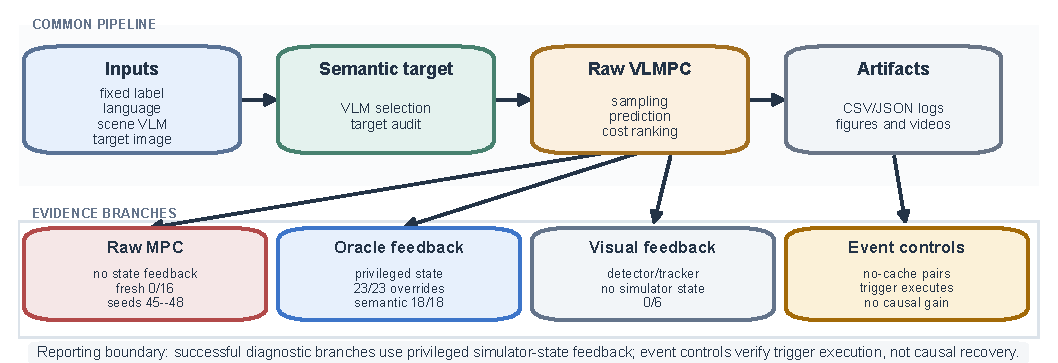
\includegraphics[width=0.98\textwidth]{method_pipeline_v9.pdf}
  \caption{Strict method overview. The common pipeline is separated from the evidence branches. Grounded original MPC and semantic MPC use privileged state feedback for execution, so their successes are reported as diagnostic stabilization rather than unmodified VLMPC success. The event-control path verifies trigger execution under matched no-cache controls, not causal recovery.}
  \label{fig:method}
\end{figure*}

\section{Experiments}
\subsection{Experiment Groups}
We organize experiments into three evidence groups.
\textbf{Raw reproduction} is the fresh four-variant, four-seed sweep of the video-prediction MPC chain without final-action state feedback; the earlier eight-run parameter ablation is retained as an explicitly archived comparison.
\textbf{Oracle-feedback diagnostics} contains grounded execution, semantic MPC, target-image grounding, and event controls that use privileged simulator state for low-level execution.
\textbf{Visual-feedback boundary} replaces the simulator-state accessor with the implemented detector/tracker path and measures the resulting boundary on six seeds. These groups are not pooled as if they were the same controller.

\subsection{Unmodified Reproduction Results}
Table~\ref{tab:unmodified} shows the fresh raw-MPC sweep. Every controller variant fails on every seed: 0/16 at the project threshold, with variant means from 0.3134 to 0.3358 and an aggregate mean of 0.3245. The failures remain 0/16 at both 0.05 and 0.10. The archived eight-run parameter ablation also remains 0/8, but it is not counted as an independent extension of the fresh seed sweep. This is the main negative result of the project and should remain visible in any final presentation.

\begin{table}[!t]
\centering
\caption{Fresh raw-MPC reproduction sweep. No privileged state feedback is used; final distance is mean $\pm$ sample SD over seeds 45--48. The archived ablation row is shown separately and is not pooled with the fresh sweep.}
\label{tab:unmodified}
\footnotesize
\begin{tabular}{@{}p{0.25\columnwidth}cccc@{}}
\toprule
Variant/suite & Runs & Succ. & Final dist. & Range \\
\midrule
Baseline & 4 & 0/4 & $0.3358{\pm}0.1099$ & 0.199--0.436 \\
Improved & 4 & 0/4 & $0.3354{\pm}0.1048$ & 0.224--0.436 \\
Literature & 4 & 0/4 & $0.3134{\pm}0.1325$ & 0.163--0.436 \\
Literature-v2 & 4 & 0/4 & $0.3134{\pm}0.1325$ & 0.163--0.436 \\
All fresh raw runs & 16 & 0/16 & $0.3245{\pm}0.1085$ & 0.163--0.436 \\
Archived ablation & 8 & 0/8 & $0.2534{\pm}0.0304$ & 0.216--0.294 \\
\bottomrule
\end{tabular}
\vspace{2pt}

\footnotesize Threshold sensitivity at 0.05/0.08/0.10 is 0/16, 0/16, 0/16 for the fresh raw sweep and 0/8, 0/8, 0/8 for the archived ablation.
\end{table}

\subsection{Feedback-Assisted Diagnostic Results}
Table~\ref{tab:diagnostic} reports the diagnostic branches. The privileged-state column changes the interpretation of the positive results. Grounded original MPC reaches 4/4 and 8/8, but all 12 runs replace 23/23 raw planner actions, so the feedback law rather than the raw planner has execution authority. The latest semantic-MPC suite reaches 18/18 only when success is defined relative to the selected target; its scope breakdown is 15/15 fixed-target controls, 1/1 natural-language instruction joint success, 1/1 target-image selected-target control, and 1/1 free scene-selection control. Only the natural-language row is instruction-evaluable; the target-image row is not an independent image-grounding test. Final selected-target distances range from 0.0297 to 0.0798; at 0.05 the selected-target control count is only 3/18. The fresh target-image matrix has no pre-satisfied cases: semantic selection and joint active control each succeed in 8/9 trials, with the yellow-pentagon seed-42 error retained. The detector/tracker visual-feedback path is a separate non-oracle test and fails in 0/6 trials. The paired semantic-fault audit is reported as a controlled repair experiment, not as evidence that natural events improve ordinary runs.

\begin{table*}[!t]
\centering
\caption{Diagnostic results and feedback source. Oracle rows use privileged simulator-state feedback and are not direct unmodified VLMPC reproductions; the visual-feedback row uses the implemented detector/tracker path without simulator-state access.}
\label{tab:diagnostic}
\scriptsize
\setlength{\tabcolsep}{2pt}
\begin{tabular}{@{}p{0.16\textwidth}p{0.06\textwidth}p{0.09\textwidth}p{0.30\textwidth}p{0.17\textwidth}p{0.12\textwidth}@{}}
\toprule
Suite & Runs & Control succ. & Evidence and semantic check & Final dist. & State \\
\midrule
Grounded controller & 4 & 4/4 & target fixed; 23/23 override & $0.0643{\pm}0.0000$ & yes \\
Grounded ablation & 8 & 8/8 & target fixed; 23/23 override & $0.0643{\pm}0.0000$ & yes \\
Event controls & 9 & 9/9 & matched controls; natural trigger 3/3 enabled, 0/3 no-event & $0.0587{\pm}0.0233$ matched & yes \\
Semantic MPC live & 18 & 18/18* & 15/15 fixed controls; language 1/1; target-image 1/1; scene 1/1 & $0.0641{\pm}0.0150$ & yes \\
Target-image matrix & 9 & 8/9 joint & semantic 8/9; no pre-satisfied & $0.0950{\pm}0.0932$ & yes \\
Visual feedback & 6 & 0/6 & detector/tracker path & $0.3160{\pm}0.1439$ & no \\
Semantic-fault audit & 12 paired & 5/6 treatment & synthetic repair 6/6; control 0/6 & $0.0639{\pm}0.0157$ treatment & yes \\
Language repeats & 9 & 9/9 joint & 3 instructions x 3 seeds; Codex no-cache & $0.0661{\pm}0.0191$ & yes \\
\bottomrule
\end{tabular}
\vspace{2pt}
\parbox{0.97\textwidth}{\footnotesize * The semantic-MPC control count is conditional on the selected target. The portable CSV separates 15 fixed-target controls (15/15), one natural-language instruction (1/1 requested-to-selected match and instruction-level joint success), one target-image interface control (1/1 selected-target control), and one free scene-selection control (1/1). Only the natural-language row is instruction-evaluable; the target-image row is not an independent image-grounding test.}
\setlength{\tabcolsep}{6pt}
\end{table*}

\begin{table*}[!t]
\centering
\caption{Condition-wise variability for the latest semantic-MPC suite. Values are mean $\pm$ sample SD of final world distance; the 18 rows are heterogeneous diagnostic runs, not 18 independent random-seed repetitions. The seed-only subset has $n=3$.}
\label{tab:variance}
\scriptsize
\begin{tabular}{@{}p{0.20\textwidth}ccccc p{0.25\textwidth}@{}}
\toprule
Condition & $n$ & Mean $\pm$ SD & $\leq0.05$ & $\leq0.08$ & Target/seed scope & Interpretation \\
\midrule
Input forms & 4 & $0.0663\pm0.0041$ & 0/4 & 4/4 & 3 forms + target image & Input-form comparison \\
Multi-target & 8 & $0.0678\pm0.0167$ & 1/8 & 8/8 & 8 target objects & Small target sweep \\
Multi-seed & 3 & $0.0587\pm0.0233$ & 1/3 & 3/3 & red moon, seeds 42/43/44 & Seed variability \\
Semantic ablation & 3 & $0.0568\pm0.0136$ & 1/3 & 3/3 & default/precise/fast & Semantic-control settings \\
All latest runs & 18 & $0.0641\pm0.0150$ & 3/18 & 18/18 & heterogeneous union & Run-level description only \\
\bottomrule
\end{tabular}
\end{table*}

\begin{figure}[!t]
  \centering
  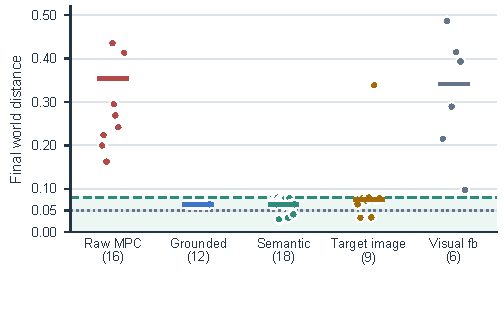
\includegraphics[width=\columnwidth]{final_distance_distribution_v9.pdf}
  \caption{Final-distance distributions across the fresh raw-MPC sweep, archived grounded diagnostics, live semantic and target-image suites, and the visual-feedback test. Each dot is one run and the horizontal segment is the within-suite median.}
  \label{fig:distance}
\end{figure}

\begin{figure}[!t]
  \centering
  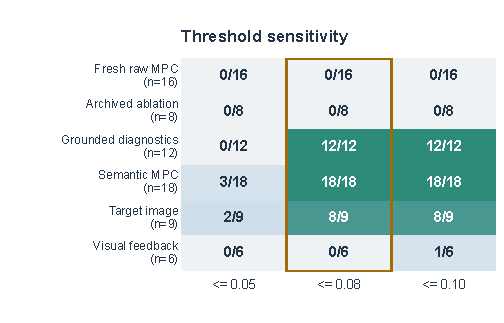
\includegraphics[width=\columnwidth]{threshold_sensitivity_v9.pdf}
  \caption{Threshold sensitivity at 0.05, 0.08, and 0.10, shown as exact selected-target control counts. The outlined column is the project threshold. Fresh raw MPC fails in 0/16 at all three thresholds; semantic MPC changes from 3/18 at 0.05 to 18/18 at 0.08. Only one row in the semantic suite is a natural-language instruction; fixed-target, target-image, and scene-selection rows are separate controls.}
  \label{fig:threshold}
\end{figure}

\subsection{Per-Run Evidence Digest}
Table~\ref{tab:perrun} gives a compact digest extracted from the portable CSVs. The full files retain seeds, labels, final distance, steps, runtime, request counts, selector metadata, and sanitized provenance. The table highlights three facts: every fresh raw-MPC run remains outside the threshold; oracle-feedback diagnostics succeed only within an explicitly privileged branch; and the first detector/tracker feedback implementation does not close that gap.

\begin{table*}[!t]
\centering
\caption{Per-run digest extracted from archived and latest CSV files. Exec. S is distance-threshold success under $\distw^{\mathrm{final}}\leq0.08$.}
\label{tab:perrun}
\scriptsize
\begin{tabular}{@{}p{0.17\textwidth}@{\hspace{4pt}}p{0.36\textwidth}@{\hspace{4pt}}p{0.13\textwidth}@{\hspace{4pt}}p{0.10\textwidth}@{\hspace{4pt}}p{0.12\textwidth}@{}}
\toprule
Suite & Final-distance summary & Range & Exec. S & Semantic/VLM evidence \\
\midrule
Fresh raw MPC & 4 variants $\times$ 4 seeds; aggregate mean $0.3245\pm0.1085$ & 0.163--0.436 & 0/16 & visual-prediction controller fails \\
Archived raw ablation & eight logged parameter settings & 0.216--0.294 & 0/8 & archived comparison \\
Grounded controller & all 0.064 & 0.064--0.064 & 4/4 & fixed target \\
Grounded ablation & all 0.064 & 0.064--0.064 & 8/8 & fixed target \\
Event controls & matched no-event/event distances identical by seed & 0.033--0.079 & 9/9 & natural trigger 3/3; no causal gain \\
Semantic MPC live & min 0.030; median 0.064; max 0.0798 & 0.030--0.0798 & 18/18 & 15/15 fixed controls; language 1/1; image 1/1; scene 1/1 \\
Target-image matrix & 8 semantic matches; one yellow-pentagon error & 0.033--0.339 & 8/9 joint & all nine are active trials \\
Visual feedback & detector/tracker feedback, seeds 45--50 & 0.097--0.487 & 0/6 & no simulator-state access \\
Semantic-fault revision audit & treatment repairs target in 6/6; control 0/6 & 0.044--0.385 & 5/6 treatment & synthetic re-query; natural count 0 \\
Language repeats & three instructions x seeds 42--44; 9/9 joint & 0.034--0.0799 & 9/9 & Codex no-cache; independent labels \\
\bottomrule
\end{tabular}
\end{table*}

\subsection{Event Re-query Evidence}
The event evidence is reported as an implementation and control supplement. The fresh 2026-09-22 set contains nine rows: three matched no-event controls, three matched event-enabled controls, and three forced scene-selection audits, all at seeds 42--44. The semantic detector uses a window of 4 and a minimum world-distance progress of 0.002. Natural event re-query fires in 3/3 event-enabled rows; the no-event and event-enabled final distances are identical seed by seed. All rows use strict no-cache mode and record zero cache hits. These controls verify trigger execution under the corrected distance scale but do not prove that natural re-query caused recovery. The separate semantic-fault audit below is deliberately evaluated against an independent true target and is reported as a controlled repair test.

\begin{table}[!t]
\centering
\caption{Fresh event re-query controls from the strict no-cache 2026-09-22 experiment.}
\label{tab:event}
\scriptsize
\setlength{\tabcolsep}{2pt}
\begin{tabular}{@{}p{0.34\columnwidth}p{0.14\columnwidth}p{0.15\columnwidth}p{0.27\columnwidth}@{}}
\toprule
Case & Natural re-query & Final dist. & Note \\
\midrule
No-event controls, seeds 42--44 & 0 & 0.0332--0.0787 & 3/3 success; 3 fresh responses \\
Event-enabled controls, seeds 42--44 & 1 each & 0.0332--0.0787 & 3/3 success; 6 fresh responses \\
Forced scene audit, seeds 42--44 & natural in 1/3; forced in all 3 & 0.0339--0.0725 & 3/3 success; 14 fresh responses \\
\bottomrule
\end{tabular}
\end{table}

\begin{table}[!t]
\centering
\caption{Controlled semantic-fault re-query audit. The wrong initial target is injected deliberately; success is measured against the independent true target.}
\label{tab:eventfault}
\scriptsize
\setlength{\tabcolsep}{2pt}
\begin{tabular}{@{}p{0.27\columnwidth}cccc@{}}
\toprule
Condition & $n$ & Semantic repair & True-target success & Final dist. \\
\midrule
No re-query control & 6 & 0/6 & 0/6 & $0.2435\pm0.0904$ \\
Synthetic re-query (Codex) & 6 & 6/6 & 5/6 & $0.0639\pm0.0157$ \\
\bottomrule
\end{tabular}
\end{table}

The treatment reaches the correct semantic target in all six paired runs, but one paired run ends just above the 0.08 threshold. The result supports a narrower statement: an explicitly forced re-query can repair a known semantic fault in this setup. It does not establish that the natural stagnation detector finds all such faults, nor that natural re-query improves ordinary successful runs.

\begin{figure}[!t]
  \centering
  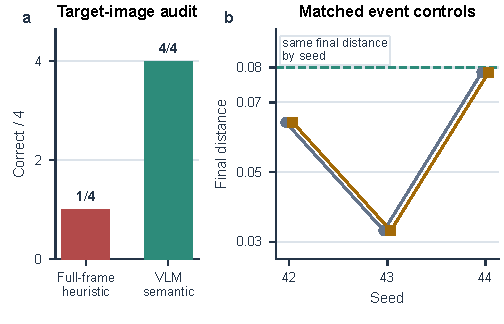
\includegraphics[width=\columnwidth]{target_event_audit_v9.pdf}
  \caption{Target-image and event-control audits. (a) The live VLM semantic selector is correct in all four audited cases, whereas the old full-frame heuristic is correct in only one. (b) Fresh strict no-cache matched controls have identical no-event and event-enabled final distances by seed; all nine rows record zero cache hits.}
  \label{fig:eventtarget}
\end{figure}

\subsection{Target-Image Selection Audit}
The target-image interface is separated into three evidence levels. The old detector/corner heuristic was fragile: it selected \emph{blue cube} in three of the four live audit cases, giving only 1/4 full-frame heuristic matches. The repaired VLM semantic selector sends both the target image and the current scene image to the configured VLM, asks for a visible scene object, and records the raw response; it matches the expected object in 4/4 audited cases. The nine-run end-to-end matrix covers three cases and seeds 42--44, with 8/9 semantic matches and 8/9 joint active successes. The four-case audit remains semantic-selection evidence, while the matrix is still a small diagnostic control study rather than a broad target-image robustness benchmark.

\begin{table}[!t]
\centering
\caption{Target-image semantic-selection audit. VLM semantic choice uses the project VLM backend with target-image and scene-image inputs.}
\label{tab:targetimage}
\scriptsize
\setlength{\tabcolsep}{1.5pt}
\begin{tabular}{@{}p{0.18\columnwidth}p{0.14\columnwidth}p{0.16\columnwidth}p{0.16\columnwidth}p{0.06\columnwidth}@{}}
\toprule
Case & Exp. & Old & VLM & OK \\
\midrule
Red-moon crop & red moon & blue cube & red moon & yes \\
Blue-cube crop & blue cube & blue cube & blue cube & yes \\
Yellow-pent. crop & yellow pentagon & blue cube & yellow pentagon & yes \\
Archived frame & red moon & blue cube & red moon & yes \\
\bottomrule
\end{tabular}
\setlength{\tabcolsep}{6pt}
\end{table}

\subsection{Revision Target-Image End-to-End Matrix}
The revision repeats the target-image path end to end for three manually specified crops and seeds 42--44. The VLM receives the target image and current scene image, selects a named scene object, and the selected target is then passed to the same semantic-MPC feedback controller. All nine trials begin outside the 0.08 threshold, so there is no pre-satisfied denominator adjustment. The yellow-pentagon run at seed 42 selects \emph{yellow star}, remains at distance 0.3386, and is retained as the negative case.

\begin{table*}[!t]
\centering
\caption{Repeated target-image end-to-end matrix. Final distance is mean $\pm$ sample SD over all runs in the case. Active trials exclude runs already within the 0.08 threshold before the first action; joint active success requires correct semantic selection and active control success.}
\label{tab:targetmatrix}
\scriptsize
\setlength{\tabcolsep}{3pt}
\begin{tabular}{@{}p{0.18\textwidth}ccccc p{0.21\textwidth}@{}}
\toprule
Target-image case & Runs & VLM semantic match & Pre-satisfied & Active joint success & Final distance & Interpretation \\
\midrule
Red moon & 3 & 3/3 & 0 & 3/3 & $0.0587\pm0.0233$ & All three trials succeed \\
Blue cube & 3 & 3/3 & 0 & 3/3 & $0.0623\pm0.0249$ & All three trials succeed \\
Yellow pentagon & 3 & 2/3 & 0 & 2/3 & $0.1640\pm0.1512$ & Seed-42 semantic error; final distance 0.3386 \\
\midrule
All cases & 9 & 8/9 & 0 & 8/9 & $0.0950\pm0.0932$ & Small diagnostic matrix, not a benchmark \\
\bottomrule
\end{tabular}
\setlength{\tabcolsep}{6pt}
\end{table*}

The complete per-run table is included in the revision target-image CSV under the sanitized supplement. This expanded matrix strengthens the end-to-end claim relative to the earlier one-run path, while the incorrect yellow-pentagon selection keeps the result bounded.

\subsection{Observed Failure Symptoms}
The failure analysis is reported as symptom taxonomy rather than causal proof. The fresh four-seed sweep fails for every raw controller variant, and the archived ablation also fails, indicating that the tested variants and parameter changes do not solve the reproduced control problem. The detector/tracker feedback path additionally fails in all six visual-feedback trials. Table~\ref{tab:symptoms} summarizes the evidence and interpretation.

\begin{table}[!t]
\centering
\caption{Observed symptoms in the final audit. These are non-exclusive observations, not single-cause proof.}
\label{tab:symptoms}
\scriptsize
\renewcommand{\arraystretch}{0.95}
\begin{tabular}{@{}p{0.25\columnwidth}@{\hspace{4pt}}p{0.68\columnwidth}@{}}
\toprule
Symptom & Evidence and interpretation \\
\midrule
Large unmodified final distance &
All 16 fresh raw-MPC runs end at 0.163--0.436, above 0.08; the reproduced video-prediction MPC chain is executable but not stable in our local setup. \\
Parameter changes do not rescue the run &
Original ablation remains 0/8 across the tested sampling and cost settings; more extensive tuning may still be possible. \\
Visual-feedback gap &
The detector/tracker feedback implementation remains 0/6 with final distance $0.3160\pm0.1439$; replacing oracle state with current visual estimates is insufficient. \\
Feedback sensitivity &
Grounded diagnostics succeed after final-action state feedback is added; this does not prove raw MPC success. \\
Semantic mismatch &
The old target-image heuristic often selects the wrong object; the repaired selector matches 4/4 audit cases and 8/9 matrix cases, with one yellow-pentagon error retained. The evidence is still small and should not be presented as broad robustness proof. \\
\bottomrule
\end{tabular}
\renewcommand{\arraystretch}{1.0}
\end{table}

\subsection{Robustness-Boundary Checks}
The robustness-edge audit is not a large benchmark, but it provides boundary evidence for the perception and target-mapping layer. Its portable CSV and four input images are included in the release artifact. The detector still identifies the red moon under target occlusion, viewpoint proxy, and brightness shift, with confidence decreasing under occlusion. Unknown or unsupported target names are safely rejected rather than mapped to arbitrary known objects. These are detector-level observations, not closed-loop robustness or real-camera generalization results.

\begin{table}[!t]
\centering
\caption{Robustness-edge audit for target detection and unknown-target handling.}
\label{tab:robust}
\footnotesize
\begin{tabular}{lcc}
\toprule
Case & Status & Confidence \\
\midrule
Original & ok & 0.902 \\
Occluded target & ok & 0.632 \\
Viewpoint proxy & ok & 0.902 \\
Brightness shift & ok & 0.900 \\
Purple pole & safe reject & -- \\
Green moon & safe reject & -- \\
Unknown target & safe reject & -- \\
\bottomrule
\end{tabular}
\end{table}

\begin{figure}[!t]
  \centering
  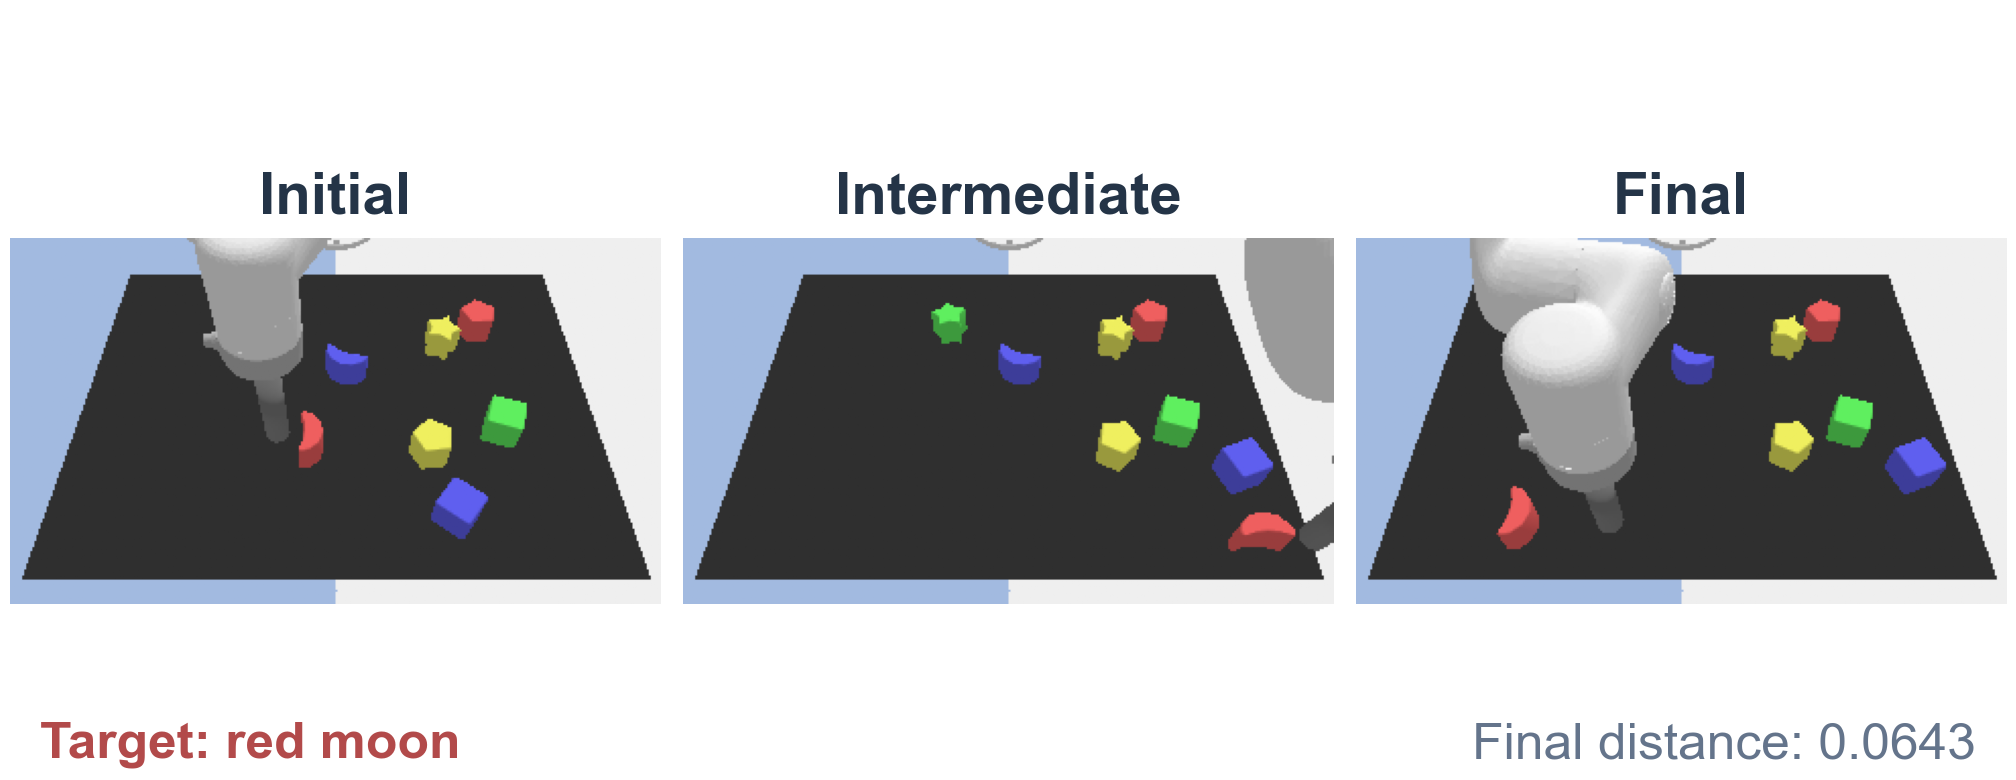
\includegraphics[width=\columnwidth]{qualitative_frames_v9.png}
  \caption{Representative frames from an oracle-feedback red-moon execution. The quantitative claims are taken from the portable run tables; the frames provide qualitative evidence of a logged Language-Table execution rather than a table-only report.}
  \label{fig:qualitative}
\end{figure}

\section{Discussion}
\subsection{Evidence Summary}
The study completes a traceable experimental workflow around the predefined evaluation protocol. The code runs the Language-Table environment, accepts multiple input forms, records GPT-5.5-based VLM responses and event triggers, evaluates raw controller variants and feedback sources, and exports sanitized per-run and aggregate evidence. The revision adds a fresh 16-run raw sweep, an 18-run live semantic suite, a nine-run target-image matrix, nine strict no-cache event controls, six detector/tracker visual-feedback runs, nine independent language repeats, and a twelve-run paired semantic-fault audit. The analysis preserves negative results rather than replacing them with only successful demonstrations.

The strongest positive evidence concerns oracle-feedback stabilization. Grounded original MPC makes the archived tasks stable under the 0.08 tolerance, but its 100\% action-replacement rate means the raw planner does not control execution. The semantic-MPC suite achieves 18/18 selected-target control successes across a heterogeneous set of targets, input forms, seeds, and settings; its auditable scope breakdown is 15/15 fixed-target controls, one natural-language instruction at 1/1, one target-image selected-target control at 1/1, and one free scene-selection control at 1/1. Only the natural-language row is instruction-evaluable, and the independent target-image matrix provides the stronger 8/9 semantic and joint active result. The new CodexCLIClient language audit adds 9/9 target-selection matches and 9/9 joint controls over three instructions and three seeds, with mean final distance $0.0661\pm0.0191$; this strengthens repeated-instruction evidence but remains small. The expanded semantic-fault audit shows 6/6 target repair and 5/6 true-target success under an explicitly forced query. These are useful diagnostic outcomes, but the 0/6 visual-feedback result shows that the oracle-to-vision replacement remains unresolved.

\subsection{Evidence Boundary}
The results do not prove that the original VLMPC paper has been reproduced at its reported performance. The fresh raw sweep fails in 0/16, and the visual-feedback controller fails in 0/6. The successful branches use privileged simulator-state feedback and are not directly comparable to the original video-prediction MPC results or published benchmarks. The semantic 18/18 count is conditional on the selected target and pools heterogeneous control scopes: 15/15 fixed-target controls, 1/1 natural-language instruction, 1/1 target-image interface control, and 1/1 scene-selection control. Only the natural-language row supports an instruction-level claim, and the independent target-image matrix is 8/9 rather than 1/1. The control result is also tolerance-dependent: semantic MPC falls from 18/18 at 0.08 to 3/18 at 0.05. Matched natural-event controls show no recovery advantage, while the paired forced-fault audit only establishes repair of a deliberately injected semantic error. Target-image grounding should therefore remain a small audited capability rather than a broad robustness claim.

\subsection{Limitations and Future Work}
The audit suggests three directions for stronger future work. First, the implemented detector/tracker visual-feedback controller should be improved rather than treated as an untested roadmap: its 0/6 result establishes the present boundary. The next evaluation should compare estimated target centroid, end-effector pose, visibility, and goal distance against simulator state using centroid error, end-effector position error, goal-distance MAE, visibility F1, and temporal consistency. Visual-only and oracle feedback should then be compared under matched seeds using final distance, success at 0.05/0.08, recovery latency, and runtime per step. The implementation route is to export synchronized RGB/state pairs, calibrate the detector/tracker on held-out seeds and perturbations, and introduce confidence-gated fallback behind the same controller interface.

Second, event-triggered re-query should be tested over more instructions, perturbations, and no-requery/forced-requery/natural-event settings. The revision's synthetic-fault audit establishes a measurable repair case but uses a forced query and therefore does not replace a natural-event causal study. A future study must induce a documented tracking or semantic failure, randomize the failure time, and compare enough matched seeds using final distance, recovery success, re-query count, recovery latency, and added VLM cost.

Third, target-image grounding should be evaluated with a larger set of image queries, cropped-object references, full-frame references, and manually verified semantic labels. These additions would convert the current diagnostic report into a stronger experimental paper without changing the interpretation of the current evidence.

\subsection{Data and Code Availability}
The public repository at \url{https://github.com/yixiaogithub66/vlmpc-language-table-reproduction-audit} and the accompanying v1.0.8 artifact include the manuscript source, authoritative 2026-09-22 and 2026-09-23 per-run and aggregate CSVs, the portable robustness-edge CSV and inputs, exact method parameters, a reproducible figure script, source and runtime-asset manifests, and an automated consistency check. The artifact deliberately excludes credentials, private endpoint addresses, local absolute paths, virtual environments, raw service logs, and third-party model weights. Reported aggregates can be recomputed from the included portable files without cached VLM responses. End-to-end reruns additionally require independently obtained detector, tracker, and video-prediction checkpoints, the `codex` CLI, and a separately configured isolated `CODEX\_HOME` profile for the CodexCLIClient, as documented in the reproduction guide.

\section{Conclusion}
This paper presents a traceable audit of a VLMPC-style Language-Table project. The fresh unmodified video-prediction MPC sweep is executable but fails in 0/16 runs, and the implemented detector/tracker visual-feedback controller fails in 0/6. Oracle-feedback diagnostics succeed under the $\distw^{\mathrm{final}}\leq0.08$ tolerance, including 18/18 selected-target semantic-MPC controls and 8/9 joint target-image trials, but these results rely on privileged simulator state. The semantic suite is explicitly partitioned into 15/15 fixed-target controls, one natural-language instruction at 1/1 instruction-level joint success, one target-image selected-target control, and one scene-selection control; the independent target-image matrix remains 8/9. A separate CodexCLIClient audit covers three instructions and seeds 42--44 with 9/9 target-selection matches and 9/9 joint controls, while the six-seed forced-fault intervention repairs 6/6 semantic states and reaches 5/6 true-target successes versus 0/6 controls. Selected-target control falls to 3/18 at 0.05. Fresh matched controls show that natural re-query executes under the corrected world-distance detector without changing final distance. The study is therefore a negative raw-reproduction audit plus bounded diagnostic evidence, not a successful unmodified VLMPC reproduction. The remaining technical problem is to close the measured oracle-to-vision gap under matched, broader task and visual-feedback evaluation.

\bibliographystyle{IEEEtran}
\bibliography{refs}

\end{document}
